\documentclass{article}
\usepackage{graphicx}

\title{4 different approaches for sorting numbers}
\author{Olcay Duzgun}

\begin{document}
\maketitle

\section{Introduction}

When it comes to sorting numbers, there are lots of different algorithms. In this essay, we will consider 4 different methods (1 bonus) and compare them with speed and efficiency.
We will be featuring Insertion sort, Radix sort, Quick sort, Heap sort and decide which sorting algorithm suits best for use cases.

\subsection{Insertion sort}
The code behind Insertion sort is rather easier than the other but first, let's dive into details.
First we start from second element of array (we count it as key) and compare with previous element.
If previous element is greater than key, we swap them.
We continue doing this for every element (excluding first one).\\
\\\textbf{Insertion sort is a stable sorting algorithm.}\\
Average complexity: $O(n^2)$\\
Best case: $O(n)$ (when array is already sorted.)\\

\subsection{Heap sort}
Heap sorting algorithm is a bit complex since its interfacing with binary tree but it's very efficient way of sorting.\\
We are generating a binary tree using our numbers.\\
Our first number will be root at the start and next element added as left element and next one is right element.
Then we add other numbers like this (adding other numbers to left as left and right again)
And we check if greater child element is greater than parent, if it is we swap them.
We continue doing this for generating max heap.
After generating final max heap,
we remove root (largest number) from heap and swap it with last element in vector.
\\\textbf{Heap sort is not a stable sorting algorithm.}\\
Complexity: $O(n * log(n))$\\

\subsection{Quick sort}
If we are looking for efficiency, Quick sort algorithm is one of the best choice among them all.
We are picking a pivot element from our array. We are using partitioning algorithm in order to divide them into two sub arrays. Then we recursively compare other elements with pivot and replace elements through it. This is how we basically implement quick sorting algorithm.\\
\\\textbf{Quick sort is not a stable sorting algorithm.}\\
Complexity: $O(n * log(n))$\\

\subsection{Radix sort}
From my testings, Radix sort didn't perform well and I couldn't find any good use case for this algorithm.
The algorithm is straight-forward to understand.
We are sorting the numbers by checking their digits. Let's say we have an array that contains 14, 62, 733, 610.
We sorting from their first digits, 610, 62, 733, 14
Then we are applying same logic for second digit and so on.
It works but didn't perform well for my use cases so it's very slow compared to other sorting algorithms.
\\\textbf{Radix sort is a stable sorting algorithm.}\\
Complexity: $O(MaxNumberOfDigits * (n + SizeOfNumber))$\\


\section{Methodology}
All of these sorting algorithms implemented using C++ programming language. I wrapped these algorithms by creating Sorting and Result classes. Which makes code very readable and clean. Also in these classes I have coded measuring elapsed time for each algorithms. It also contains a test system to make sure algorithm is working as it supposed to. 

\section{Results}
As of my observations, quick sort is the fastest algorithm for sorting numbers with $O(n * log(n))$ complexity.
Insertion sort is doing great job when it comes to handle low amount of array size but it cannot remain its performance good if array size is large enough.
Heap sorting algorithm is also a good choice but still slower than quick sort.
Radix sort is not that comparable to others but still faster than Insertion sort if the array has large set.

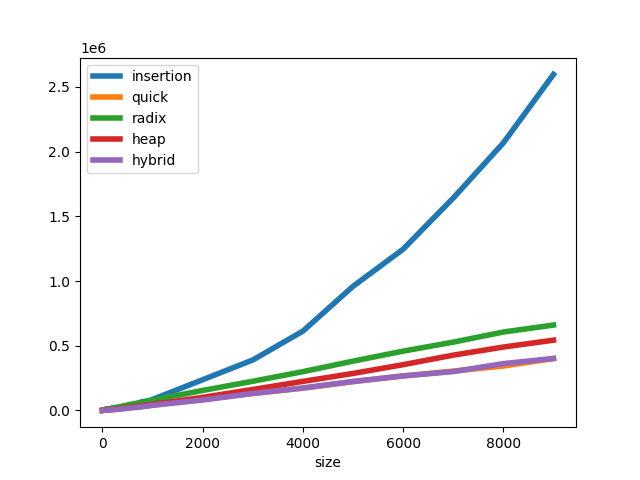
\includegraphics[width=0.8\linewidth,height=0.4\textheight]{../data/full.png}

\end{document}